\documentclass[a4paper,11pt]{article}

\usepackage{../../zyancamlec}

\usepackage{tikz-feynhand}

\def\ntripos{Mathematical Tripos}
\def\npart{III}
\def\ncourse{Algebraic Topology}
\def\nscourse{AlgTop}
\def\nlecturer{I.\ Smith}
\def\nterm{Michaelmas}
\def\nyear{2020}

\begin{document}
	\maketitlepage
	\preliminaries

	\section*{Course Information}

	Algebraic Topology permeates modern pure mathematics and theoretical physics. This course will focus on (co)homology, with an emphasis on applications to the topology of manifolds. We will cover singular and cellular (co)homology; degrees of maps and cup-products; cohomology with compact supports and Poincar\'e duality; and Thom isomorphism and the Euler class. The course will not specifically assume any knowledge of algebraic topology, but will go quite fast in order to reach more interesting material, so some previous exposure to chain complexes (e.g. simplicial homology) would certainly be helpful.
	
	\section*{Pre-requisites}

	Basic topology: topological spaces, compactness and connectedness, at the level of Sutherland’s book. Some knowledge of the fundamental group would be helpful though not a requirement. Hatcher’s book and Bott and Tu’s book are especially recommended for accompanying the course, but there are many other suitable texts.

	\newpage
	\tableofcontents
	\newpage
	\maintext
	\setcounter{section}{-1}
	\section{Introduction} \lecnr{1}
	
	\emph{Algebraic Topology} concerns the \emph{connectivity} properties of topological spaces.

	\begin{defi}
		A space $X$ is \emph{path-connected} if for $p,q\in X$, $\exists \gamma: [0,1] \to X$ continuous with $\gamma(0) = p, \gamma(1) = q$. 
	\end{defi}

	\needfig{1}

	\begin{ex}
		$\mathbb{R}$ is path-connected; $\mathbb{R} \backslash \{0\}$ is not.
	\end{ex}

	\begin{cor}[The intermediate value theorem]
		If $f : \mathbb{R} \to \mathbb{R}$ is continuous and $x < y$ satisfy $f(x)<0, f(y)>0$ then $f$ takes the value 0 on $[x,y]$.
	\end{cor}

	\begin{proof}
		Otherwise, $f^{-1}(-\infty,0)\cup f^{-1}(0,\infty)$ disconnects $[x,y]$, \#. 
	\end{proof}

	\begin{defi}
		Let $X,Y$ be topological spaces. We say maps $f_0, f_1 : Y \to X$ are \emph{homotopic} if $\exists F : Y \times [0,1] \to X$ continuous such that
		\[
			F|_{Y \times \{0\}} = f_0, \qquad F|_{Y \times \{1\}} = f_1
		\]
		
		We write $f_0 \simeq f_1$ (or $f_0 \underset{F}{\simeq} f_1)$.
	\end{defi}
	\needfig{2}

	\begin{exer}
		(On example sheet 1) $\simeq$ is an equivalence relation on the set of maps from $Y$ to $X$.
	\end{exer}

	\begin{nt}
		$X$ is \emph{path-connected} iff every two maps $\{\text{point}\} \to X$ are homotopic.
	\end{nt}

	\begin{defi}
		$X$ is \emph{simply-connected} if every two maps $S^1 \to X$ are homotopic.
	\end{defi}

	\begin{nt}
		We often denote
		\[
			S^1 = \{z \in \mathbb{C} : \abs{z} = 1\}, \qquad S^n = \{x\in \mathbb{R}^{n+1} : \norm{x} = 1\}
		\]
	\end{nt}

	\begin{ex}
		$\mathbb{R}^2$ is simply connected; $\mathbb{R}^2 \backslash \{0\}$ is not.

		From complex analysis we know $\gamma: S^1 \to \mathbb{R}^2 \backslash \{0\}$ has a \emph{winding number} or \emph{degree} $\deg (\gamma) \in \mathbb{Z}$, for which
		\begin{enumerate}
			\item If $\gamma_n (t) = e^{2\pi \mathrm{i} n t}$ then $\deg (\gamma_n) = n$;
			\item $\deg(\gamma_1) = \deg(\gamma_2)$ if $\gamma_1 \simeq \gamma_2$.  
		\end{enumerate} 
		\needfig{3}

		For \emph{differentiable} $\gamma$, 
		$$\deg(\gamma) = \int_\gamma \frac{\dd{z}}{z}.$$
	\end{ex}
	
	\begin{cor}[Fundamental theorem of algebra]
		Every non-constant complex polynomial has a root.
	\end{cor}

	\begin{proof}
		Let $f(z) = z^n + a_1 z^{n-1} + \cdots + a_n$ be non-constant and WLOG monic. Suppose $f(z) \neq 0, \forall z \in \mathbb{C}$, let $\gamma_R (t):= f\left( R e^{2\pi \mathrm{i} t} \right)$ so that $\gamma_R : S^1 \to \mathbb{R}^2 \backslash \{0\}$. We know that
		\[
			\gamma_0 \text{ is constant} \quad \Rightarrow\quad \deg(\gamma_0) = 0 \quad \Rightarrow\quad \deg(\gamma_R) = 0, \quad \forall R
		\]
		However, if we take $R \gg \sum_i \abs{a_i}$, let $f_s(z) = z^n + s \left( a_1 z^{n-1} + \cdots + a_n \right)$ with $0 \leq s \leq 1$. On the circle $\abs{z} = R$, $f_s(z) \neq 0, \forall s$.

		Therefore, if $\gamma_{R,s}(t) := f_s\left( R e^{2\pi \mathrm{i} t} \right)$ then we have $\gamma_{R,1} = \gamma_R$ and $\gamma_{R,0} : t \mapsto R^n e^{2\pi \mathrm{i} n t}$.
		
		Clearly, we have
		\[
			\deg(\gamma_{R,1}) = 0 \neq n = \deg(\gamma_{R,0}) 
		\]
		as non-constant property suggests $n \neq 0$. This is a \#.
	\end{proof}

	\begin{defi}
		$X$ is \emph{$k$-connected} if every two maps $S^i \to X$ are homotopic whenever $i \leq k$.
	\end{defi}

	\begin{ex}
		$\mathbb{R}^n$ is $(n-1)$-connected; $\mathbb{R}^n \backslash \{0\}$ is not. Maps $S^{n-1} \to \mathbb{R}^n \backslash \{0\}$ have a homotopy-invariant degree $\in \mathbb{Z}$ and deg(inclusion) = 1, deg(constant) = 0. (We'll prove it later.)
	\end{ex}

	\begin{cor}[Brouwer's theorem]
		For closed unit ball $\bar{B}^n = \{x\in \mathbb{R}^n : \norm{x}\leq 1\}$, any map $f : \bar{B}^n \to \bar{B}^n$ has a fixed point.
	\end{cor}

	\begin{proof}
		Suppose $f$ has no fixed point. Let $\gamma_R (v) := Rv - f(Rv)$ where $0 \leq R \leq 1$ and $v \in S^{n-1} = \partial \bar{B}^n$. Our assumption suggests $\gamma_R$ takes values in $\mathbb{R}^n \backslash \{0\}$.

		According to homotopy invariance, as $\gamma_0$ is constant, we have $\deg(\gamma_0) = 0$ hence $\deg(\gamma_1) = 0$.
		
		Let $\gamma_{1,s}(v) := v - s f(v)$ for $0 \leq s \leq 1$. Then $\gamma_{1,1} = \gamma_1$ and $\text{image}(\gamma_{1,s}) \subseteq \mathbb{R} \backslash \{0\}$ as $\norm{v} = 1, \norm{s f(v)} = \abs{s}\norm{f(v)} < 1$ if $s < 1$.
		
		Therefore, we have $\deg(\gamma_{1,0}) = \deg(\gamma_{1,1}) = 0$ by homotopy invariance. However, the inclusion $\gamma_{1,0}$ should have degree 1, thus \#.
	\end{proof}

	\begin{defi}
		$f: X \to Y$ is a \emph{homotopy-equivalence} if $\exists g : Y \to X$ such that $f \cpf g \simeq \id_Y, g \cpf f \simeq \id_X$. (We call $g$ a ``homotopy inverse'' for $f$.)
	\end{defi}

	\begin{nt}
		The homotopy equivalence can be shown as an equivalence relation on spaces.
	\end{nt}

	\begin{ex}
		If $X,Y$ are homeomorphic they are trivially homotopy equivalent: simply by taking $g = f^{-1}$.
	\end{ex}

	\begin{ex}
		$\mathbb{R}^n \backslash \{0\} \simeq S^{n-1}$. 
		
		Let
		\[
			f: \mathbb{R}^n \backslash \{0\} \to S^{n-1}, \quad v \xmapsto{f} \frac{v}{\norm{v}}
		\]
		\[
			g: S^{n-1} \hookrightarrow \mathbb{R}^n \backslash \{0\} \text{ by inclusion}
		\]
		Then
		\[
			f \cpf g = \id_{S^{n-1}}, \qquad g \cpf f \underset{F}{\simeq} \id_{\mathbb{R}^n \backslash \{0\}}
		\]
		via the homotopy
		\[
			F(t,v) = tv + (1-t) \frac{v}{\norm{v}}
		\]
		\needfig{4}
	\end{ex}

	\begin{ex}
		$\{0\} \xhookrightarrow{\sim} \mathbb{R}^n$ is a homotopy equivalence. (Check!)
	\end{ex}

	\begin{defi}
		If a space $X \simeq \{\text{point}\}$ we say $X$ is \emph{contractible}. 
	\end{defi}

	Talking about all these, we emphasise that
	\[
		\boxed{\text{Algebraic topology is the study of topological spaces up to homotopy equivalence.}}
	\]
	
	The main idea is that: homeomorphism is too delicate as a relation, but homotopy equivalence keeps track of ``essential'' topological information. More precisely, we assign
	\begin{align*}
		\{\text{Spaces}\} & \to \{\text{Groups}\}\\
		\{\text{Maps of spaces}\} & \to \{\text{Homomorphisms of groups}\}
	\end{align*}
	so we get algebraic invariants. (They are defined for \emph{all} spaces, but have more structure and use/interest for ``nicer'' spaces.)

	The classical first attempt of algebraic topology would be \emph{homotopy theory}. One can \emph{concatenate} loops:
	\needfig{5}
	for
	\[
		\gamma * \tau (t) = \begin{cases}
			\gamma(2t),& t \leq \frac{1}{2}\\
			\tau(1 - 2t),& t \geq \frac{1}{2}
		\end{cases}
	\]
	which leads to
	\[
		\{\text{Maps }S^1 \xrightarrow{\gamma} X\} / \simeq \quad  \longrightarrow \quad \pi_1(X,x_0)
	\]
	where $\gamma$ fixes $\gamma(0) = x_0 \in X$ and the homotopies preserve $x_0$; 
	\needfig{6}
	$\pi_1$ is called the \emph{fundamental group} on which the group operation is the concatenation $(\gamma, \tau) \mapsto \gamma * \tau$. 
	
	Similarly, for higher dimensions \needfig{7}

	giving
	\[
		\pi_n (X, x_0) = \{\text{based maps}\} / \simeq
	\]
	called the \emph{$n$-th homotopy group} of $X$.

	The issue is that these homotopy groups are very hard to compute. E.g.\ $\pi_n (S^2, x_0)$ is not known $\forall n$.
	
	There is even \emph{no} simply connected manifold (a space $X$ locally homeomorphic to $\mathbb{R}^n$) of dimension $> 0$ with $\pi_n (X)$ known $\forall n$!
	
	Therefore, we will do something else: \emph{(co)homology}.

	It is algebraically harder to set up, yet the computational gain is worth it. Please note that computing cohomology of ``harder'' spaces (e.g.\ $\text{Diff}(X), \text{Emb}(X,Y), \dots$) is still very hard.

	Some general remarks:
	\begin{itemize}
		\item Algebraic topology is all about being able to \emph{compute}. It is important to do lots of examples;
		\item Our ``nice spaces'' are \emph{manifolds} and indeed \emph{smooth manifolds} --- some of these will overlap with the course \emph{Differential Geometry} which will be useful. 
	\end{itemize}

	\newpage
	\section{Homology and Cohomology}
	\subsection{Chain \& Cochain Complexes} \lecnr{2}

	We will define invariants of spaces in two stages:
	\begin{enumerate}
		\item Associate to $X$ a (co)chain complex;
		\item Take the (co)homology of that complex. 
	\end{enumerate}

	\begin{defi}
		A \emph{chain complex} $(C_* , \partial)$ is a sequence of abelian groupd and homomorphisms
		\[
			\cdots \to C_{n+1} \xrightarrow{\partial_{n+1}} C_n \xrightarrow{\partial_n}C_{n-1} \xrightarrow{\partial_{n-1}} C_{n-2} \to \cdots
		\]
		such that $\partial_{n-1} \cpf \partial_n = 0, \forall n$. We write this as ``$\partial^2 = 0$''.

		The \emph{homology group} $H (C_*, \partial)$ is the graded group 
		\[
			H_n (C_*) := {\ker (\partial_n)}/{\im (\partial_{n+1})}.
		\]
	\end{defi}
	\begin{nt}
		We may call $\partial$ the ``differential'' or ``boundary map''.
	\end{nt}

	\begin{defi}
		A \emph{cochain complex} is a sequence of abelian groups and homomorphisms $(C^*, \partial)$
		\[
			\cdots \to C^{n-1} \xrightarrow{\partial^{n-1}} C^n \xrightarrow{\partial^n} C^{n+1} \xrightarrow{\partial^{n+1}} C^{n+2} \to \cdots
		\]
		such that $\partial^n \cpf \partial^{n-1} = 0, \forall n$ (``$\partial^2 = 0$'' again).

		The \emph{cohomology groups} $H(C^*, \partial)$ are
		\[
			H^n (C^*) := {\ker(\partial^n)}/{\im(\partial^{n-1})}.
		\]
	\end{defi}

	\begin{nt}
		Here we introduce some terminologies.
		\begin{itemize}
			\item Elements of $\ker \partial : C_n \to C_{n-1}$ are called \emph{cycles};
			\item Elements of $\im \partial : C_{n+1} \to C_n$ are called \emph{boundaries};
			\item Elements of $\ker \partial : C^n \to C^{n+1}$ are called \emph{cocycles}. 
		\end{itemize}
	\end{nt}
	\begin{exer}
		Try to define \emph{coboundary}.
	\end{exer}

	\begin{nt}
		For convenience (we are lazy!), we write all $\partial_i$ and $\partial^i$ as $\partial$ (or occasionally $\partial,\partial^*$).
	\end{nt}

	\begin{defi}
		The elements of $H_*(C_*)$ are \emph{homology classes} and those of $H^*(C^*)$ are \emph{cohomology classes}.
	\end{defi}

	\begin{defi}
		A \emph{chain map} between chain complexes $(C_*,\partial)$ and $(D_*,\partial)$ is a sequence of homomorphisms $f_n : C_n \to D_n$ such that $\forall n$ the following commutes:
		\begin{center}
			\begin{tikzcd}
				\cdots \arrow[r] & C_n \arrow[r, "\partial"] \arrow[d, "f_n"] & C_{n-1} \arrow[r] \arrow[d,"f_{n-1}"] & \cdots \\
				\cdots \arrow[r] & D_n \arrow[r, "\partial"] & D_{n-1} \arrow[r] & \cdots 
			\end{tikzcd}
		\end{center}
		i.e.\ $f_{n-1} \cpf \partial_n^{C_*} = \partial_n^{D_*} \cpf f_n$. 
	\end{defi}

	\begin{exer}
		Define a \emph{cochain map} of cochain complexes.
	\end{exer}

	\begin{lem}
		A chain map $f_* : C_* \to D_*$ induces homomorphisms
		\[
			(f_n)_\star : H_n (C_*) \to H_n(D_*)
		\]
		for each $n$.
	\end{lem}

	\begin{proof}
		Let $[a] \in H_n (C_*)$, so $a$ is represented by a cycle $\alpha \in C_n$. Use the commutativity of the diagram in the above definition, we have
		\[
			\partial(f_n (\alpha)) = f_{n-1}(\underbrace{\partial \alpha}_{0}) = 0
		\]
		so $f_n (\alpha)$ is a cycle.

		Define
		\[
			f_\star [a] := [f_n(\alpha)] \in H_n(D_*).
		\]
		
		We made a choice of representing cycle $\alpha$. But if $[a]$ is represented by $\alpha$ and $\alpha'$, then
		\[
			\alpha - \alpha' \in \im(\partial_{n+1}: C_{n+1} \to C_n).
		\]
		
		Say $\alpha - \alpha' = \partial \tau$, then
		\[
			f_n (\alpha) - f_n(\alpha') = f_n (\alpha - \alpha') = f_n (\partial\tau) = \partial(f_{n+1}(\tau)).
		\]
		
		Thus
		\[
			[f_n (\alpha)] = [f_n (\alpha') + \partial f_{n+1}(\tau)] = [f_n (\alpha')]
		\]
		as $[\im(\partial)] = 0$ in $H_*$.
		
		So $f_{\star}$ is well-defined, and easy to see it's a homomorphism.
	\end{proof}

	\begin{exer}
		If $C_*, D_*, E_*$ are chain complexes and $f : C_* \to D_*$, $g: D_* \to E_*$ are chain maps then $\{g_n \cpf f_n : C_n \to E_n\}_n$ defines a chain map and
		\[
			(\dagger)\begin{cases}
				(g \cpf f)_\star = g_\star \cpf f_\star,\\
				(\id)_\star = \id \text{ on $H(C_*)$ themselves}.
			\end{cases}
		\]
	\end{exer}

	Discussing all these, our goal is associating to space $X$ (co)chain complexes $C_*(X), C_*(X)$ such that a map $f : X \to Y$ yields (co)chain maps
	\[
		C_* (X) \xrightarrow{f_*} C_* (Y)
	\]
	and
	\[
		C^* (Y) \xrightarrow{f^*} C^*(X).
	\]
	
	\begin{nt}
		$(\dagger)$ means that we can say we have a \emph{functor} $\mathbf{Top} \to \mathbf{Groups}$, $X \mapsto H_\star(X)$ where the categories are 
		\[
			\mathbf{Top} = (\text{spaces, continuous maps})\text{ and }\mathbf{Groups} = (\text{abelian groups, homomorphisms}). 
		\]
		
	\end{nt}

	Our complexes $C_*, C^*$ will have the benefit that they are ``intrinsic'' but will be huge and unwieldy. We will 
	\begin{enumerate}
		\item Prove structure theorems to help compute these;
		\item Find ``smaller'' complexes later for nice spaces (e.g.\ CW-complexes).
	\end{enumerate}

	\begin{defi}
		The \emph{standard simplex} is defined as 
		\[
			\Delta^n := \left\{(t_0, \cdots, t_n)\in \mathbb{R}^{n+1} : t_i \geq 0, \sum_i t_i = 1\right\}.
		\]
		
		The $i$-th \emph{face} of $\Delta^n$ is
		\[
			\Delta^n_i := \{\vb t \in \Delta^n : t_i = 0\}.
		\]
	\end{defi}

	\begin{nt}
		There exists canonical homeomorphism $\Delta^{n-1} \xrightarrow{\delta_i} \Delta^n_i$ such that
		\[
			(t_0, \cdots, t_{n-1}) \mapsto (t_0, \cdots, t_{i-1}, 0, t_{i+1}, t_{n-1}).
		\]
	\end{nt}

	\begin{defi}
		If $X$ is a space, a \emph{singular $n$-simplex in $X$} is a map $\sigma: \Delta^n \to X$. The \emph{singular chain complex} $(C_*(X),\partial)$ has
		\[
			C_n (X) := \left\{ \sum_{i=1}^N n_i \sigma_i : N<\infty, n_i \in \mathbb{Z}, \sigma_i: \Delta^n \to X\right\},
		\]
		the free abelian groups on the singular $n$-simplices in $X$, and
		\[
			\partial: C_n (X) \to C_{n-1}(X), \quad \sigma \mapsto \sum_{i=0}^n (-1)^i (\sigma \cpf \delta_i)
		\]
		which extends linearly.
	\end{defi}

	\begin{nt}
		The $n+1$ ordered points $\{v_i\}_{0 \leq i \leq n} \subseteq \mathbb{R}^{n+1}$ determine an $n$-simplex if $\{v_i - v_0 : 1 \leq i \leq n\}$ are linearly independent. Take their convex hull and set 
		\[
			\sigma: \Delta^n \to \mathbb{R}^{n+1}, \quad \vb t \mapsto \sum_{i=0}^n t_i v_i.
		\]
		
		We orient the edges as $v_i \to v_j$ if $i < j$. Write $\underbrace{[v_0 \cdots v_n]}_{\sigma}$ for this $n$-simplex, then
		\[
			\partial \sigma := \sum_{i=0}^n (-1)^i \sigma\bigg|_{[v_0 \cdots \hat{v}_i \cdots v_n]}
		\]
		where the hat means omission.
	\end{nt}

	\needfig{8}

	\begin{lem}
		$\partial^2=0$.
	\end{lem}

	\begin{proof}
		\[
			\partial (\partial \sigma) = \sum_{j<i} (-1)^i (-1)^j \sigma\bigg|_{[v_0 \cdots \hat{v}_j \cdots \hat{v}_i \cdots v_n]} + \sum_{j>i} (-1)^i (-1)^{j-1} \sigma\bigg|_{[v_0 \cdots \hat{v}_i \cdots \hat{v}_j \cdots v_n]}
		\]
		
		Exchange the $i$ and $j$ in the second term, the two terms cancel.
	\end{proof}

	\begin{defi}
		The \emph{singular homology} is defined as $H_*(X) = H_*(x; \mathbb{Z}):= H(C_*(X),\partial)$.
	\end{defi}
	\begin{nt}
		This is \emph{trivially} a homeomorphism invariant of $X$ since we only used the notion of continuous map to $X$ to define it.
	\end{nt}

	\begin{ex}
		\needfig{9}

		We take four 1-simplices to form a closed path as shown.

		The annulus to the left has 
		\[
			\partial(\sigma_1 + \sigma_2 + \sigma_3 + \sigma_4) = 0
		\]
		and to the right, the connected space also has
		\[
			\partial(\gamma_1 + \gamma_2 + \gamma_3 + \gamma_4) = 0.
		\]
		
		But what we can confirm is that 
		\[
			\gamma_1 + \gamma_2 + \gamma_3 + \gamma_4 \in \im(\partial)
		\]
		e.g.\ $\partial(\tau) = [v_0 v_1]-[v_0 v_2] + \underbrace{[v_1 v_2]}_{\gamma_3}$. This means that the homology class defined by such $\sum_i \gamma_i$ is 0. However, for $\sigma$ it should be non-zero --- the singular homology probes `holes' in a space.
	\end{ex}

	\begin{defi}
		The \emph{sigular cochain complex} $C^*(X)$ has
		\[
			C^n(X) := \Hom(C_n(X), \mathbb{Z})
		\]
		\[
			\partial^*: C^n (X) \to C^{n+1}(X), \qquad (\partial^* \psi)(\sigma) := \psi(\partial\sigma),\quad \sigma\in C_{n+1}(X)
		\]
		
		Then 
		\[
			\partial^* (\partial^* \psi)(\sigma) = \partial^*(\psi(\partial \sigma)) = \psi (\partial(\partial\sigma)) = 0.
		\]
		i.e. $(\partial^*)^2 = 0$: this is indeed a cochain complex. 
	\end{defi}

	\begin{nt}
		$H^*(X;\mathbb{Z}) := H^*(C^*(X),\partial^*)$ is \emph{singular cohomology} of $X$. 
		
		$H^*(X;\mathbb{Z})\ \cancel{\cong}\ \Hom(H_*(X),\mathbb{Z})$ in general.
		
		We bothered to define such cochain complex and cohomology because later we will show cohomology is a ring (which has better algebraic properties) while homology is not.
	\end{nt}
	
	\begin{nt}[Rough idea]
		We have several \emph{heuristic} ideas (don't take too seriously!):
		\begin{itemize}
			\item $\partial^2 = 0$ means ``the boundary of the boundary vanishes'';
			\item $H_i(X)$ will probe ``$i$-dimensional holes/regions'' in $X$;
			\item $H^i (X)$ will be a rule associating an integer to an $i$-dimensional region of $X$.
		\end{itemize}
	\end{nt}

	\lecnr{3}

	\begin{rmk}
		Let $f : X \to Y$ be continuous. If $\sigma: \Delta^n \to X$ then $f \cpf \sigma : \Delta^n \to Y$, meaning that $f$ induces homomorphisms
		\[
			f_n : C_n (X) \to C_n(Y)
		\]
		and by $f\cpf (\sigma \cpf \delta_i) = (f \cpf \sigma) \cpf \delta_i$, we have
		\[
			f \cpf \left( \sigma\big|_{\text{$i$-th face}} \right) = (f \cpf \sigma)\big|_{\text{$i$-th face}}
		\]
		Thus $f_* : C_* (X) \to C_*(Y)$ is a chain map
		\begin{center}
			\begin{tikzcd}
				C_n(X) \arrow[r, "\partial"] \arrow[d, "f_n"] & C_{n-1}(X) \arrow[d, "f_{n-1}"]\\
				C_n(Y) \arrow[r, "\partial"] & C_{n-1}(Y)
			\end{tikzcd}
		\end{center}
		also giving homomorphisms
		\[
			f_\star : H_{\star} (X) \to H_{\star}(Y).
		\]
	\end{rmk}

	\begin{exer}
		Show that
		\[
			(f\cpf g)_* = f_* \cpf g_*, \qquad (\id)_* = \id.
		\]
	\end{exer}

	\begin{nt}
		$f: X \to Y$ also induces 
		\[
			f^* : C^* (Y) \to C^*(X), \quad (f^* \psi) (\sigma) := \psi(f \cpf \sigma)
		\]
		and
		\[
			f^\star : H^\star(Y) \to H^\star(X)
		\]
		where $\sigma : \Delta^n \to X$ and $\psi: C_n(Y) \to \mathbb{Z}$.
		
		Note that in the language of category theory, we say ``cohomology is a contravariant functor''.
	\end{nt}

	\subsection{Homology of the Circle}

	So far, what can we compute?

	\begin{lem}
		Let $X$ be a point. Then the singular homology is
		\[
			H_i (\{\text{pt}\}) = \begin{cases}
				\mathbb{Z} & i=0\\
				0 & \text{otherwise}
			\end{cases}
		\]
	\end{lem}

	\begin{proof}
		For each $n\geq 0$, there exists a unique $n$-simplex in $X$, $\sigma_n : \Delta^n \to \{\text{pt}\}$, the constant map. So $C_*(\{\text{pt}\})$ is
		\begin{center}
			\begin{tikzcd}
				\cdots \arrow[r, ""] & C_3 \arrow[r, ""] \arrow[d, equal, ""] & C_2 \arrow[r, ""] \arrow[d, equal, ""] & C_1 \arrow[r, ""] \arrow[d, equal, ""] & C_0 \arrow[d, equal, ""]\\
				\cdots \arrow[r, "+1"] & \mathbb{Z} \arrow[r, "0"] & \mathbb{Z} \arrow[r, "+1"] & \mathbb{Z} \arrow[r, "0"] & \mathbb{Z}  
			\end{tikzcd}
		\end{center}
		
		We find
		\[
			\partial \sigma_1 = \partial (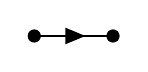
\begin{tikzpicture}
				\begin{feynhand}
					\vertex [dot] (a) at (0,0) {};
					\vertex [dot] (b) at (1,0) {};
					\propag [fer] (a) to [] (b);
				\end{feynhand}
			\end{tikzpicture}) = \bullet - \bullet = 0
		\]
		and 
		\[
			\partial \sigma_2 = \sigma_2 \cpf \delta_0 - \sigma_2 \cpf \delta_1 + \sigma_2 \cpf \delta_2 = \sigma_1
		\]
		
		Thus by induction,
		\[
			\partial \sigma_n = \begin{cases}
				\sigma_{n-1} & n \text{ even}\\
				0 & n \text{ odd}
			\end{cases}
		\]

		Then if we see how these relate kernels and images at different $n$, our result is clear.
	\end{proof}
	
	

	\begin{exer}
		Check the cohomology 
		\[
			H^i(\{\text{pt}\}) \cong \begin{cases}
				\mathbb{Z} & i = 0\\
				0 & \text{otherwise}
			\end{cases}
		\]
	\end{exer}

	There is basically only one other computation we can do from the definitions.

	\begin{lem}
		If $X = \bigsqcup_{\alpha \in I} X_\alpha$ is a disjoint union of path-components, then
		\[
			H_i(X) \cong \bigoplus_{\alpha \in I} H_i (X_\alpha), \quad \forall i.
		\]
	\end{lem}

	\begin{proof}
		Any continuous map $\sigma : \Delta^i \to X$ has image in one $X_\alpha$ and then all the faces of $\sigma$ lie in the \emph{same} $X_\alpha$. So
		\[
			C_*(X) = \bigoplus_\alpha C_*(X_\alpha)
		\]
		compatibly with the differential.
	\end{proof}

	\begin{lem}
		If $X$ is path-connected (and non-empty), $H_0 (X) \cong \mathbb{Z}$.
	\end{lem}

	(An aside note: We sometimes write $\pi_0(X)$ for the \emph{set} of path-components of $X$.)

	\begin{proof}
		Define 
		\[
			\varepsilon: C_0 (X) \to \mathbb{Z}, \quad \sum_{\text{finite}} n_i \sigma_i \mapsto \sum_i n_i
		\]
		called the \emph{augmentation}, where $\sigma_i : \{\text{pt}\} \to X$ are 0-simplices in $X$. As $X \neq \0$, $\varepsilon$ is surjective.
		
		If $\tau : \Delta^1 \to X$, 
		
		\needfig{10-1}

		we have
		\[
			\varepsilon(\partial \tau) = \varepsilon(v_1 - v_0) = 0
		\]
		so
		\[
			\im(\partial: C_1 \to C_0) \subseteq \ker(\varepsilon)
		\]
		i.e.\ $\varepsilon$ defines $H_0(X) \to \mathbb{Z}$.

		So far we didn't use path-connectivity. But suppose $\sum_i n_i \sigma_i \in \ker(\varepsilon)$. Fix a base point $p \in X$ and for every $i$ we pick
		\[
			\tau_i : \Delta^1 \cong [0,1] \to X, \quad \begin{cases}
				\tau_i (1) = \sigma_i (\Delta^0)\\
				\tau_i (0) = p
			\end{cases}
		\]

		\needfig{10-2}

		and we have
		\[
			\partial \left( \sum_i n_i \tau_i \right) = \sum_i n_i \sigma_i - \cancelto{\text{\tiny 0}}{\left( \sum_i n_i \right)} p 
		\]
		as $\sum_i n_i \sigma_i \in \ker(\varepsilon)$, so
		\[
			\ker(\varepsilon) \subseteq \im(\partial)
		\]
		and we identify
		\[
			\varepsilon : C_0(X) / \im(\partial) =: H_0 (X) \xrightarrow{\cong} \mathbb{Z}.
		\]
		
	\end{proof}

	\paragraph{\underline{Informal Picture}} 
	Recall $\sigma : \Delta^1 \cong [0,1] \to X = \text{Annulus}$ has $\partial \sigma = \sigma(1) - \sigma(0) = 0$, so $\sigma$ defines $[\sigma]\in H_1(X)$.
	
	\needfig{11-1}

	We would hope this is non-zero, as we can't ``see'' a way to fill in $\sigma$ with 2-simplices. (Contrast with the case where $\tau \in \im(\partial)$.)

	\needfig{11-2}

	However, $C_i(X)$ is uncountably generated for all $i$, and is very hard to control.

	The question is: how do we rule out \emph{all} configurations of 2-simplices? Or, are there any other representations for $[\sigma]\in H_1(X)$? 

	\paragraph{\underline{Informal Conjecture}} In the realm of ``nice'' spaces, there is \emph{nothing else} you can compute from the definition!

	(Co)homology is rendered useful by a collection of structural theorems: we will state these and see how to use them and then return to prove them later.

	\begin{thm}[Homotopy invariance]
		If $f : X \to Y$ and $g: X \to Y$ are homotopic, then 
		\[
			f_\star = g_\star : H_\star(X) \to H_\star(Y) \quad \text{and} \quad f^\star = g^\star : H^\star(Y) \to H^\star(X).
		\]
	\end{thm}

	\begin{cor}
		If $X \simeq Y$ (homotopy-equivalent), then 
		\[
			H_\star (X) \cong H_\star (Y) \quad \text{and} \quad H^\star(X) \cong H^\star(Y).
		\]
	\end{cor}

	\begin{proof}
		There exists $f: X \to Y$ and $g : Y\to X$ such that $g \cpf f \simeq \id_X$ and $f \cpf g \simeq \id_Y$ thus $(f_\star)^{-1} = g_\star$ are isomorphisms.
	\end{proof}

	Thus (co)homology is insensitive to ``inessential'' deformations of a space.

	\begin{cor}
		\[
			H_* (\mathbb{R}^n) \cong \begin{cases}
				\mathbb{Z} & * = 0\\
				0 & \text{otherwise}
			\end{cases}
		\]
		for every $n$. And similar for $H^*$.
	\end{cor}

	But we still cannot compute very much... 

	\begin{defi}
		An \emph{exact sequence} is a (co)chain complex with vanishing\\(co)homology:
		\[
			\cdots \to C_{n+1} \xrightarrow{\partial_{n+1}} C_n \xrightarrow{\partial_n} C_{n-1} \to \cdots
		\]
		such that $\ker(\partial_n) = \im(\partial_{n+1}), \forall n$. 
	\end{defi}

	\begin{nt}
		There are some additional terminologies/facts:
		\begin{itemize}
			\item Given homomorphisms \[
				A \xrightarrow{f} B \xrightarrow{g} C
			\]
			say this is \emph{exact at $B$} if $\ker g = \im f$;
			\item If \[
				0 \to A \xrightarrow{f} B \to 0
			\]
			is exact, we have $A \cong B$;
			\item A \emph{short exact sequence} is one of shape \[
				0 \to A \xrightarrow{f} B \xrightarrow{g} C \to 0
			\]
			which says $f$ is injective and $g$ is surjective.
		\end{itemize}
	\end{nt}

	\begin{thm}[Mayer-Vietoris]
		If $X = A \cup B$ with $A,B$ open, there are ``Mayer-Vietoris boundary homomorphisms''
		\[
			\partial_{\text{MV}} : H_{i+1}(X) \to H_i (A \cap B)
		\]
		yielding a ``long'' exact sequence (LES):
		\[
			\cdots \to H_{i+1}(X) \xrightarrow{\partial_{\text{MV}}} H_i (A\cap B) \xrightarrow{(i_{A\star},i_{B\star})} H_i(A) \oplus H_i(B) \xrightarrow{j_{A\star}-j_{B\star}} H_i(X) \to \cdots
		\]
		where $i_{A\star}, j_{A\star}$, etc.\ are induced from certain inclusion maps in the commutative diagram below
		\begin{center}
			\begin{tikzcd}
				A \cap B \arrow[r,hookrightarrow, "i_A"] \arrow[d, hookrightarrow, "i_B"] & A \arrow[d, hookrightarrow, "j_A"]\\
				B \arrow[r, hookrightarrow, "j_B"] & X
			\end{tikzcd}
		\end{center}
		and $\partial_{\text{MV}}$ is defined algebraically, not associated to a map of spaces.
	\end{thm}

	\begin{rmk}
		Suppose $\sigma \in C_{i+1}(X)$ is a \emph{cycle} and $\sigma = \alpha + \beta$, $\alpha \in C_{i+1}(A), \beta \in C_{i+1}(B)$ for \emph{chains} $\alpha,\beta$ (i.e.\ $\partial \alpha, \partial\beta$ need not vanish). Then $\partial \alpha = - \partial \beta$ and $$\partial_{\text{MV}} [\sigma] = [\partial \alpha]$$ as $\partial \alpha = - \partial \beta$ gives $\partial \alpha \in C_{i}(A \cap B)$. 

		\needfig{12}
	\end{rmk}

	\begin{addendum}
		The MV sequence is \emph{natural}. If $X = A \cup B$ and $Y = C \cup D$ and $f: X \to Y$ has $f(A) \subseteq C$ and $f(B) \subseteq D$ (under maps of pairs), then there are homomorphisms of exact exact sequences
		\begin{center}
			\begin{tikzcd}
				\cdots \arrow[r, ""] & H_{i+1}(X) \arrow[r, "\partial^X_{\text{MV}}"] \arrow[d, "f_\star"] & H_i (A\cap B) \arrow[r, ""] \arrow[d, "f_\star"] & H_i(A) \oplus H_i(B) \arrow[r, ""] \arrow[d, "f_\star"] & H_i(X) \arrow[r, ""] \arrow[d, "f_\star"] & \cdots\\
				\cdots \arrow[r, ""] & H_{i+1}(Y) \arrow[r, "\partial^Y_{\text{MV}}"] & H_i(C\cap D) \arrow[r, ""] & H_i(C) \oplus H_i(D) \arrow[r, ""] & H_i(Y) \arrow[r, ""] & \cdots
			\end{tikzcd}
		\end{center} 
		such that all squares commute.
	\end{addendum}

	\begin{rmk}
		There is a MV sequence in cohomology, also natural:
		\[
			\partial^*_{\text{MV}}: H^i (A \cap B) \to H^{i+1}(X)
		\]
		such that
		\[
			\cdots \to H^i(X) \xrightarrow{(j_A^\star,j_B^\star)} H^i(A) \oplus H^i(B) \xrightarrow{i_A^\star - i_B^\star} H^i(A \cap B) \xrightarrow{\partial^*_{\text{MV}}} H^{i+1}(X) \to \cdots
		\]
		is \emph{exact}.
	\end{rmk}

	Finally, we get something to compute: the homology of the circle.

	\begin{prop}
		\[
			H_i (S^1) \cong \begin{cases}
				\mathbb{Z} & i = 0,1\\
				0 & \text{otherwise}
			\end{cases}	
		\]
		and 
		\[
			H^i (S^1) \cong \begin{cases}
				\mathbb{Z} & i = 0,1\\
				0 & \text{otherwise}
			\end{cases}	
		\]
	\end{prop}
	\begin{proof}
		Choose $A$ and $B$ such that $S^1 = X = A \cup B$ and $A,B$ are open intervals, $A \cap B$ is the union of 2 disjoint open intervals, shown as in the figure below
		
		\needfig{13}

		So, we have $A \simeq \{\text{pt}\} \simeq B$ and $A \cap B \simeq \underbrace{\{p\} \sqcup \{q\}}_{S^0, \text{0-sphere}}$. 

		Recall that 
		\[
			H_* (\mathbb{R}) \cong \begin{cases}
				\mathbb{Z} & * = 0\\
				0 & \text{otherwise}
			\end{cases}
		\]
		and $\mathbb{R} \simeq \{\text{pt}\}$. By homotopy invariance, we know $H_*(A), H_*(B), H_*(A \cap B)$.

		If we take the MV sequence for $i \geq 2$, we have
		\[
			\cancelto{\text{\tiny 0}}{H_i (A) \oplus H_i(B)} \to H_i(S^1) \to \cancelto{\text{\tiny 0}}{H_{i-1}(A\cap B)} \quad \Rightarrow \quad H_i(S^1) = 0.
		\]
		
		For $i = 1$, we have
		\begin{center}
			\begin{tikzcd}
				\cancelto{\text{\tiny 0}}{H_1 (A\cap B)} \arrow[r, ""] & \cancelto{\text{\tiny 0}}{H_1(A)\oplus H_1(B)} \arrow[r, ""] & H_1(S^1) \arrow[dll,out=0, in=180, ""]\\
				H_0(A \cap B) \arrow[r, "{(i_A, i_B)}"] \arrow[d, equal, "\cong"] & H_0(A)\oplus H_0(B) \arrow[r, "(j_A - j_B)"] \arrow[d, equal, "\cong"] & H_0(S^1) \arrow[d, equal, "\cong"]\\
				\mathbb{Z} \oplus \mathbb{Z} \arrow[r, dashrightarrow, "\alpha"] & \mathbb{Z}\oplus \mathbb{Z} \arrow[r, dashrightarrow, "\beta"] & \mathbb{Z}
			\end{tikzcd}
		\end{center}

		Recall that for some path-connected space $Z$, $H_0(Z)$ is a free abelian group on $\pi_0 (Z)$ (the set of path-components), and indeed this is generated by
		\[
			\sigma : \{\text{pt}\} \to Z
		\]
		for any choice of point in each component.

		So from
		\[
			H_0 (A \cap B) = \mathbb{Z}\expval{p} \oplus \mathbb{Z} \expval{q} \xrightarrow{(i_A,i_B)} \mathbb{Z} \oplus \mathbb{Z}
		\]
		we identify the map
		\[
			\alpha : (a,b) \mapsto (a+b , a+b)
		\]
		and from
		\[
			\mathbb{Z} \oplus \mathbb{Z} \xrightarrow{j_A - j_B} H_0 (S^1)
		\]
		we have
		\[
			\beta : (u,v) \mapsto u-v.
		\]
		
		The exactness of the sequence gives
		\[
			H_1(S^1) \cong \ker(\alpha) \cong \mathbb{Z}
		\]
		which is generated by 
		\[
			(1,-1) \equiv (p, -q) \in H_0(A) \oplus H_0(B).
		\]
	\end{proof}

	\lecnr{4}

	The same method as for computing $H_*(S^1)$ shows for $n$-spheres:

	\begin{prop}
		\[
			H_j(S^n) \cong \begin{cases}
				\mathbb{Z} & j = 0,n\\
				0 & \text{otherwise}
			\end{cases}
		\]
		and
		\[
			H^j(S^n) \cong \begin{cases}
				\mathbb{Z} & j = 0,n\\
				0 & \text{otherwise}
			\end{cases}
		\]
	\end{prop}
	\begin{proof}
		This time, let's do the cohomology computation. Consider the following figure.

		\needfig{14}

		For the above choice of $A,B$, homotopy invariance and induction gives $H^*(A), H^*(B)$ and $H^*(A\cap B)$. 

		MV now gives
		\begin{center}
			\begin{tikzcd}
				&\cdots \arrow[r, ""] & H ^{i-1}(S ^{n-1}) \arrow[dll,overlay,out=0,in=180 , ""]\\
				H ^{i}(S ^{n}) \arrow[r, ""] & \cancelto{\text{\tiny 0}}{H ^{i}(\mathbb{R}^{n}) \oplus H ^{i}(\mathbb{R}^{n})} \arrow[r, ""] & H ^{i}(S ^{n-1}) \arrow[dll,overlay,out=0,in=180, ""] \\
				H ^{i+1}(S ^{n}) \arrow[r, ""] &  \cancelto{\text{\tiny 0}}{H ^{i+1}(\mathbb{R}^{n}) \oplus H ^{i+1}(\mathbb{R}^{n})} \arrow[r, ""] & \cdots 
			\end{tikzcd}
		\end{center}
		and we find for $i > 0$, 
		\[
			0 \to H^i (S ^{n-1}) \to H ^{i+1} (S^n) \to 0
		\]
		is exact, giving
		\[
			H^i(S ^{n-1}) \cong H ^{i+1}(S^n),
		\]
		which we can use in the induction.

		Now for the base case $i = 0$,
		\begin{center}
			\begin{tikzcd}
				H^0 (S^n) \rar & H^0(\mathbb{R}^n) \oplus H^0(\mathbb{R}^n) \rar \arrow[d,equal, "\cong"] & H^0(S ^{n-1}) \rar \arrow[d, equal, "\cong"] & H^1 (S^n) \rar & 0\\
				& \mathbb{Z} \oplus \mathbb{Z} \rar & \mathbb{Z} & &
			\end{tikzcd}
		\end{center}
		Note that here we use $n > 1$ as $S^0$ is not connected. 

		As we showed before that for \emph{path-connected} $X$
		\[
			H_0(X) \cong \mathbb{Z} \quad \text{generated by} \quad \underbrace{\sigma_0 : \{\text{pt}\} \to X}_{\in C_0(X)}. 
		\]
		
		In example sheet 1, you should've proved
		\[
			H^0 (X) \cong \mathbb{Z} \quad \text{generated by} \quad \psi : C_0(X) \to \mathbb{Z},\  \underbrace{\psi(\sigma) = 1}_{\in C^0(X)}, \forall \sigma : \{\text{pt}\} \to X.
		\]
		
		so in
		\begin{center}
			\begin{tikzcd}
				H^0 (S^n) \rar \arrow[d,equal, "\cong"] & H^0(\mathbb{R}^n) \oplus H^0(\mathbb{R}^n) \rar \arrow[d,equal, "\cong"] & H^0(S ^{n-1}) \rar \arrow[d, equal, "\cong"] & H^1 (S^n) \rar & 0\\
				\mathbb{Z} & \mathbb{Z} \oplus \mathbb{Z} \arrow[r, twoheadrightarrow, "\alpha"] & \mathbb{Z} & &
			\end{tikzcd}
		\end{center}
		with $\alpha(p,q) = p + q$ which is surjective, we have
		\[
			H^1(S^n) = 0.
		\]
		
		And now we've computed enough to complete the induction.
	\end{proof}

	\begin{cor}
		$$\mathbb{R}^m \cong \mathbb{R}^n \quad \Leftrightarrow \quad m = n.$$
	\end{cor}
	\begin{proof}
		We have
		\begin{center}
			\begin{tikzcd}
				\mathbb{R}^m \cong \mathbb{R}^n \arrow[r,Rightarrow, shorten <= 1ex, shorten >= 1ex, ""] & \mathbb{R}^m \backslash \{0\} \arrow[d,dash, "\simeq"]  \ar[r,equal, "\cong"] & \mathbb{R}^n \backslash \{0\} \arrow[d,dash, "\simeq"]\\
				& S ^{m-1} \arrow[r, dash, "\simeq"] & S ^{n-1}
			\end{tikzcd}
		\end{center}
		which gives
		\[
			H_*(S ^{m-1}) \cong H_* (S ^{n-1})
		\]
		thus
		\[
			m = n.
		\]
	\end{proof}

	This homeomorphism invariance of dimension was an early success of the subject.

	Recall there are \emph{space-filling curves}
	\[
		\gamma : [0,1] \to [0,1]^2
	\]
	continuous and surjective!

	\subsection{Degrees} 

	\begin{lem}
		A map $f : S^n \to S^n$ has a \emph{degree}
		\[
			\deg(f) \in \mathbb{Z}
		\]
		and if $g \simeq f$, $\deg(g) = \deg(f)$.
	\end{lem}

	\begin{proof}
		$f$ induces
		\begin{center}
			\begin{tikzcd}
				f_\star: H_n(S^n) \arrow[r, ""] \arrow[d,equal, "\cong"] & H_n(S^n) \arrow[d,equal, "\cong"]\\
				 \mathbb{Z} \arrow[r,dashed, "\text{homomorphism}"] & \mathbb{Z}
			\end{tikzcd}
		\end{center}
		where the homomorphism in general is multiplication by an integer, and this defines $\deg(f)$.

		Also, $g \simeq f$ suggests $g_\star = f_\star$ hence $\deg(g) = \deg(f)$.
	\end{proof}

	\begin{nt}
		{\color{red}\underline{Caveat!}} Use the same isomorphism (as there is an automorphism of $\mathbb{Z}$ by multiplying $-1$) on both sides: make sure $\deg(f)$ is defined but not just up to a change in sign.
	\end{nt}

	\begin{exer}
		Check $$\deg(f \cpf g) = \deg(f) \deg(g).$$
	\end{exer}

	\begin{ex}
		$\deg(\id) = 1$.
	\end{ex}

	\begin{cor}
		If $f$ is a homeomorphism, $\deg(f) \in \{\pm 1\}$. 
	\end{cor}

	\begin{ex}
		$\deg(\text{constant map}) = 0$. 
	\end{ex}
	\begin{proof}
		The constant map $S^n \to S^n$ such that $f(x) = p \in S^n, \forall n$ factorises as 
		\[
			S^n \to \{\text{pt}\} \to S^n
		\]
		so that $f_\star$ factorises through the \emph{zero} group
		\begin{center}
			\begin{tikzcd}
				H_n (S^n) \rar \arrow[d,equal, "\cong"] & H_n(\{\text{pt}\}) \rar \arrow[d,equal, "\cong"] & H_n(S^n) \arrow[d,equal, "\cong"]\\
				\mathbb{Z} \rar \arrow[rr,blue,dashed,bend right, "f_\star"] & 0 \rar & \mathbb{Z}
			\end{tikzcd}
		\end{center}
		thus the homomorphism associates to degree zero.
	\end{proof}

	\begin{nt}
		Combining with $S ^{n-1} \simeq \mathbb{R}^n \backslash \{0\}$, this fills in details for results from lecture 1 on Brouwer's theorem.
	\end{nt}

	\begin{lem}
		A matrix $A \in \Og(n+1)$ acts on $H_n(S^n, \mathbb{Z})$ by multiplication by $\det (A)$.
	\end{lem}
	\begin{proof}
		$\Og(n+1)$ has two path-connected components, so by homotopy invariance of degree, it suffices to show reflection in a hyperplane has degree $-1$.

		The following figure shows the settings.

		\needfig{15}

		We denote the reflection in hyperplane $H$ as
		\[
			\text{refl}_H : S^n \to S^n
		\]
		which induces reflection in $H'$ for the boundary $\partial L$ of invariant hemisphere $L$
		\[
			\text{refl}_{H'} : S ^{n-1} \to S ^{n-1}.
		\]
		
		We computed $H_*(S^n)$ by MV, and now we can use the decomposition which is $\text{refl}_H$-invariant. The naturality of MV gives
		\begin{center}
			\begin{tikzcd}
				0 \rar & H_n(S^n) \arrow[d,blue, "\text{refl}_H"] \arrow[r, "\cong"] & H _{n-1}(S ^{n-1}) \arrow[d,blue, "\text{refl}_{H'}"] \rar & 0\\
				0 \rar & H_n(S^n) \arrow[r, "\cong"] & H _{n-1}(S ^{n-1}) \rar & 0
			\end{tikzcd}
		\end{center}

		Inductively, it suffices to treat the case $n=1$.

		So, consider a circle shown below.

		\needfig{16}

		Our former MV computation of $H_*(S^1)$ gave
		\begin{center}
			\begin{tikzcd}
				0 \rar & H_1(S^1) \rar & H_0 (\{p\} \sqcup \{q\}) \arrow[d,equal, "\cong"] \rar["\alpha"] & H_0(A) \oplus H_0(B) \arrow[d,equal, "\cong"]\\
				& & \mathbb{Z} \oplus \mathbb{Z} \arrow[r, "{(u,v)\mapsto (u+v,u+v)}"] & \mathbb{Z} \oplus \mathbb{Z}
			\end{tikzcd}
		\end{center}
		and
		\[
			H_1(S^1) = \ker(\alpha) \cong \mathbb{Z}\expval{(1,-1)}
		\]
		is generated by $\expval{p} - \expval{q}$, so as $\text{refl}_H$ exchange $p,q$, it acts on $H_1(S^1)$ by $-1$.
	\end{proof}

	\begin{cor}
		\
		\begin{enumerate}
			\item The antipodal map $a_n : S^n \to S^n, x \mapsto -x$ has degree $(-1)^{n+1}$;
			\item If $f: S^n \to S^n$ has no fixed point, $f \simeq a_n$;
			\item If $G$ acts freely on $S ^{2k}$, then $G \leq \mathbb{Z}/2$.
		\end{enumerate}
	\end{cor}
	\begin{proof}
		\ 
		\begin{enumerate}
			\item \begin{tikzcd}[baseline=1.45em]
				a_n : S^n \quad \rar[shorten <= -2ex] \arrow[d,hookrightarrow, "\subseteq"]& S^n \arrow[d,hookrightarrow, "\subseteq"]\\
				\mathbb{R}^{n+1} \arrow[r, "{v\mapsto -v}"] & \mathbb{R}^{n+1}
			\end{tikzcd} is a composition of $(n+1)$ reflections as
			\[
				(v_1, \cdots, v _{n+1}) \mapsto (-v_1,\cdots, - v _{n+1}).
			\]
			\item We will show $f(x)\neq g(x), \forall x$ suggests $f \simeq a_n \cpf g$.
			
			Consider 
			\[
				x \xmapsto{\varphi_t} \frac{t f(x) - (1-t) g(x)}{\norm{t f(x) - (1-t) g(x)}}
			\]
			for $0 \leq t \leq 1$.

			Note that 
			\[
				t f(x) - (1-t)g(x) \neq 0 \quad \text{or} \quad t = \frac{1}{2} \text{ and } f(x) = g(x)
			\]
			so
			\[
				f = \varphi_1 \simeq \varphi_0 = a_n \cpf g.
			\]
			\item See example sheet 1.
		\end{enumerate}
	\end{proof}

	We borrow a concept from Differential Topology.
	\begin{defi}
		A \emph{vector field} on $S^n$ is a map
		\[
			v: S^n \to \mathbb{R}^{n+1}
		\]
		such that
		\[
			\forall x \in S^n, \quad \expval{x, v(x)} = 0
		\]
		where $\expval{\cdot,\cdot}$ is the Euclidean inner product on $\mathbb{R}^{n+1}$.
	\end{defi}

	\begin{nt}
		This is a global section of the tangent bundle $TS^n \to S^n$.
	\end{nt}

	\begin{prop}[Hairy ball theorem]
		$S^n$ has a nowhere-vanishing vector field if and only if $n$ is odd.
	\end{prop}

	\begin{proof}
		If $n = 2k-1$, set 
		\[
			v(x_1,y_1, \cdots, x_k, y_k) := (-y_1,x_1,\cdots, -y_k, x_k)
		\]
		and we are done.

		Suppose $n$ is even and for contradiction that such $v$ exists. Normalisation is a map
		\[
			\frac{v}{\norm{v}} : S^n \to S^n.
		\]
		as the unit vectors are also elements of $S^n$.

		Consider 
		\[
			v_t(x):= (\cos t)x + (\sin t) \frac{v}{\norm{v}}(x),
		\]
		we find $\norm{v_t(x)} = 1, \forall t$, and
		\[
			v_0 = \id, \quad v_\pi = - \id = a_n
		\]
		so
		\[
			\id _{S^n} \simeq a_n \quad \Rightarrow \quad \deg(\id) = \deg(a_n) \quad \Rightarrow \quad 1 = (-1)^{n+1}
		\]
		which requires odd $n$, contradiction.
	\end{proof}

	\subsection{The Klein Bottle} \lecnr{5}

	We should do one computation which involves \emph{knowing} the maps (not just on $H_0$) in an exact sequence, and not just that the sequence is exact. For this we want to compute the (co)homology for a Klein bottle.

	The \emph{Klein bottle} $K$ is obtained from gluing two M\"obius bands together.

	\needfig{17}

	\begin{lem}
		$$H_j(K; \mathbb{Z})\cong \begin{cases}
			\mathbb{Z} & j=0\\
			\mathbb{Z} \oplus \mathbb{Z}/2 & j=1\\
			0 & \text{otherwise}
		\end{cases}$$
	\end{lem}

	\begin{proof}
		We make decomposition shown in the following figure.

		\needfig{18}

		Apply MV to $K = A \cup B$, $A,B$ and $A\cap B$. Note that one can show $A, B \simeq S^1$ and $A \cap B \simeq S^1$.

		The essential part of the LES is 
		\begin{center}
			\begin{tikzcd}
				& & \mathbb{Z} \rar & \mathbb{Z} \oplus \mathbb{Z}\\
				0 \rar & H_2(K) \rar & H_1(A\cap B) \arrow[u,equal, "\cong"'] \arrow[r, "\psi"] & H_1(A)\oplus H_1(B) \arrow[u,equal, "\cong"'] \arrow[dll, out=0,in=180,overlay, ""]\\
				& H_1(K) \arrow[r, "0"] & H_0(A \cap B) \arrow[d,equal, "\cong"] \arrow[r,hookrightarrow, ""] & H_0(A) \oplus H_0(B) \arrow[d,equal, "\cong"]\\
				& & \mathbb{Z} \rar & \mathbb{Z} \oplus \mathbb{Z}
			\end{tikzcd}
		\end{center}

		The exactness of the sequence gives 
		\[
			H_1 (K) = (\mathbb{Z}\oplus \mathbb{Z}) / \im \psi \quad \text{and} \quad H_2(K) \cong \ker \psi.
		\]
		The key claim here is 
		\[
			\psi(1) = (2,2).
		\]
		(Note that $(\mathbb{Z}\oplus \mathbb{Z})/(2,2)\cong \mathbb{Z} \oplus \mathbb{Z}/2$.)

		To prove the claim, we use the fact that
		\begin{enumerate}
			\item $A\cap B \simeq$ the boundary circle of central M\"obius band;
			\item $A \simeq$ the core circle of central M\"obius band.
		\end{enumerate}
		to pick the generators as following
		
		\needfig{19}

		We have
		\[
			H_1(A\cap B) = \mathbb{Z} \expval{v+w} \quad \text{and} \quad H_1(A) = \mathbb{Z}\expval{\sigma_1 + \sigma_2}.
		\]
		
		From the figure it is easy to see
		\[
			v \mapsto \sigma_1 + \sigma_2 \quad \text{and} \quad w \mapsto \sigma_1 + \sigma_2.
		\]
		and we're done.
	\end{proof}

	\begin{rmk}
		We could define $C_k(X; G) := \{\sum _{\text{finite}} a_i \sigma_i : a_i \in G, \sigma_i : \Delta^k \to X\}$ for \emph{any} abelian group $G$, with the same differential $\partial$. These lead to the \emph{singular homology with coefficients in $G$} $H_*(X;G)$.
	\end{rmk}

	\begin{exer}
		Show that
		\[
			H_j(S^1; \mathbb{Z}/2) \cong \begin{cases}
				\mathbb{Z}/2 & j \in \{0,1\}\\
				0 & \text{otherwise}
			\end{cases}
		\]
		and
		\[
			H_i(\{\text{pt}\};\mathbb{Z}/2)\cong\begin{cases}
				\mathbb{Z}/2 & i=0\\
				0 & \text{otherwise}
			\end{cases}	
		\]
	\end{exer}

	In the previous sequence, if we compute $H_*(K;\mathbb{Z}/2)$, we get
	\begin{center}
		\begin{tikzcd}
			0 \rar & H_2(K;\mathbb{Z}/2) \rar & H_1(A \cap B; \mathbb{Z}/2) \arrow[r, "\psi"] \arrow[d,equal, "\cong"] & H_1(A; \mathbb{Z}/2) \oplus H_1(B; \mathbb{Z}/2) \arrow[d,equal, "\cong"]\\
			& & \mathbb{Z}/2 \arrow[r, "{1 \mapsto (2,2)\equiv (0,0)}"] & \mathbb{Z}/2 \oplus \mathbb{Z}/2
		\end{tikzcd}
	\end{center}
	so that $\psi$ vanishes for $H_*(-; \mathbb{Z}/2)$. Thus
	\[
		H_i (K; \mathbb{Z}/2) \cong \begin{cases}
			\mathbb{Z}/2 & i=0\\
			\mathbb{Z}/2 \oplus \mathbb{Z}/2 & i=1\\
			\mathbb{Z}/2 & i = 2\\
			0 & \text{otherwise}
		\end{cases}
	\]
	
	It's also instructive to think about cohomology (in $\mathbb{Z}$ coefficients, still) in this example: $K = A\cup B$, $A,B\simeq S^1$, $A \cap B \simeq S^1$ as before. The cohomology MV sequence look like
	\begin{center}
		\begin{tikzcd}
			H^0 (A\cap B)\rar &[-1em] H^1(K) \arrow[r, "{(j_A^\star, j_B^\star)}"] & H^1 (A) \oplus H^1 (B) \arrow[d,equal, "\cong"] \arrow[r, "i_A^\star - i_B^\star"] & H^1(A\cap B) \arrow[d,equal, "\cong"] \rar &[-1em] H^2(K) \rar &[-1em] 0\\
			& & \mathbb{Z}\oplus \mathbb{Z} \arrow[r, "\alpha"] & \mathbb{Z} & &
		\end{tikzcd}
	\end{center} 
	where one can check
	\[
		\alpha: (a,b)\mapsto 2(a-b).
	\]
	
	So we have
	\[
		H^2(K) \cong \mathbb{Z}/2.
	\]
	
	(Contrast: $H_2(K) = 0$ if we use $\mathbb{Z}$ coefficients.)

	\begin{nt}
		The important point here to raise is that: there were \emph{many} ways we could have cut up $K$. For example, we can decompose $K$ into a disc and its complement.

		\needfig{20}

		We set $A = \text{disc}$ and $B = K \backslash \text{disc}$. Then it can be shown $B \simeq S^1 \vee S^1$,
		where $S^1 \vee S^1$ is the wedge of two circles: that they join at one point. 

		$H_*(A)$ is shown before, $H_*(B)$ is computable by using MV sequence. Then we can find $H_*(K)$ using MV under such decomposition.

		In some cases, some decomposition will give easier algebra than others.
	\end{nt}

	\subsection{Homotopy Invariance}

	Now we should pay some debts: proving homotopy invariance.

	\begin{defi}
		Chain maps $f_* : C_* \to D_*$ and $g_* : C_* \to D_*$ are said to be \emph{chain homotopic} if there exists $P_n : C_n \to D _{n+1}$ such that 
		\[
			P _{n-1} \cdot \partial_n ^{C_*} \pm \partial _{n+1}^{D_*} \cdot P_n = f_n - g_n.
		\]

		This can be shown by a commutative diagram:
		\begin{center}
			\begin{tikzcd}
				\cdots \rar &[-1em] C _{n+1} \arrow[d, "f_{n+1} - g_{n+1}"'] \arrow[r, "\partial"] & C _{n} \arrow[d, "f_{n} - g_{n}"] \arrow[r, "\partial"] \arrow[dl,blue, "P_{n}"] & C _{n-1} \arrow[d, "f_{n-1} - g_{n-1}"] \arrow[r, ""] \arrow[dl,blue, "P_{n-1}"] &[-1em] \cdots\\[2em]
				\cdots \rar & D_{n+1} \arrow[r, "\partial"'] & D_n \arrow[r, "\partial"'] & D_{n-1} \rar & \cdots
			\end{tikzcd}
		\end{center}
	\end{defi}

	\begin{lem}
		If $f_* : C_* \to D_*$ and $g_* : C_* \to D_*$ are chain homotopic, then
		\[
			f_\star = g_\star : H_i(C_*, \partial) \to H_i(D_*, \partial), \quad \forall i
		\]
		i.e.\ chain homotopic maps induce the same map on homology.
	\end{lem}

	\begin{proof}
		Since $f_*$ and $g_*$ are chain homotopic, i.e.\ the following diagram commute
		\begin{center}
			\begin{tikzcd}
				C _{n+1} \arrow[d,dashed] \arrow[r,dashed] & C _{n} \arrow[d, "f_{n} - g_{n}"] \arrow[r, "\partial"] \arrow[dl,blue, "P_{n}"] & C _{n-1} \arrow[d,dashed] \arrow[dl,blue, "P_{n-1}"]\\
				D_{n+1} \arrow[r, "\partial"'] & D_n \arrow[r,dashed] & D_{n-1}
			\end{tikzcd}
		\end{center}
		so
		\[
			P _{n-1} \partial \pm \partial P_n = f_n - g_n.
		\]
		
		Let $\alpha \in C_n$ be a cycle, i.e.\ $\partial \alpha = 0$. Then we have $\partial f_n(\alpha) = f _{n-1}(\partial \alpha) = 0$ and
		\[
			f_\star [\alpha] := [f_n (\alpha)].
		\]

		Consider
		\[
			f_n (\alpha) - g_n (\alpha) = (f_n - g_n) (\alpha) = P _{n-1} (\partial \alpha) \pm \partial P_n (\alpha) = \partial P_n (\alpha) \in \im(\partial),
		\]
		so
		\[
			[f_n(\alpha)] = [g_n(\alpha)] \in H(D_*).
		\]
	\end{proof}

	\begin{exer}
		Show that chain homotopy is an equivalence relation on chain complexes and chain maps.
	\end{exer}
	
	\begin{thm}[Homotopy invariance, v2]
		If $f \simeq g : X \to Y$ then $f_* \simeq g_* : (C_*(X),\partial) \to (C_*(Y),\partial)$. 
	\end{thm}
	
	\begin{proof}
		$f \simeq g$ suggests there exists
		\[
			F : X \times [0,1]\to Y \quad \text{s.t.} \quad F\big|_{X \times \{0\}} = f, \ F\big|_{X \times \{1\}} = g.
		\]
		
		So, if
		\[
			\begin{rcases}
				i_0 : X \hookrightarrow X \times [0,1] & x \mapsto (x,0)\\
				i_1 : X \hookrightarrow X \times [0,1] & x \mapsto (x,1)
			\end{rcases} \quad f = F \cpf i_0, \quad g = F \cpf i_1.
		\]
		then 
		\[
			f_* = g_* \quad \text{if} \quad (i_0)_* = (i_1)_*
		\]
		and it suffices to prove
		\[
			(i_0)_* \simeq (i_1)_* : C_*(X) \to C_*(X\times[0,1]).
		\]
		
		We want $P : C_n(X) \to C _{n+1} (X \times [0,1])$. The idea is that $P$ is a \emph{prism operator}. It gives a ``universal way'' of cutting up $\Delta^n \times [0,1]$ into $(n+1)$-simplices
		\begin{align*}
			C_n(X) \qquad & \to \qquad C _{n+1}(X\times [0,1])\\
			\sigma: \Delta^n \to X \quad& \mapsto \quad \text{lin. comb. of } \sigma \times \id : \Delta^n \times [0,1] \to X \times [0,1].
		\end{align*}
		
		The equation $\partial P \pm P \partial = (i _{1*} - i _{0*})$ says
		\[
			\text{``boundary of prism $=$ prism on boundary $+$ top $-$ bottom''}
		\]

		\needfig{21}

		The details of the proof are not very illuminating, so we will be quite terse... (See Hatcher's book for details.)

		Label base of prism by $[v_0\cdots v_n]$ and top by $[w_0 \cdots w_n]$.

		\paragraph{Claim 1.} $\sigma _{n+1}^i = [v_0 \cdots v_i w_i \cdots w_n]$ is an $(n+1)$-simplex and 
		\[
			\Delta^n \times [0,1] = \bigcup _{i=0}^n \sigma _{n+1}^i.
		\]

		It should be intuitive from the pictures. We won't prove this, see Hatcher's book.

		Define
		\[
			P: \begin{dcases}
				C_n (X)  & \to \qquad C _{n+1} (X \times [0,1])\\
				\sigma  & \mapsto \qquad \sum _{i=0}^n (-1)^i (\sigma \times 1)\big|_{[v_0\cdots v_i w_i\cdots w_n]} = \sum _{i=0}^n (-1)^i (\sigma \times 1) \cpf \sigma _{n+1}^i.
			\end{dcases}
		\]
		
		\paragraph{Claim 2.} $\partial P + P \partial = (i_1)_* - (i_0)_*$.

		For this, one can check
		\begin{align*}
			\partial P \sigma & = \sum _{j \leq i} (-1)^i (-1)^j (\sigma \times 1)\big|_{[v_0 \cdots \hat{v}_j \cdots v_i w_i \cdots w_n]}\\
			& \quad + \sum _{j \geq i} (-1)^i (-1)^{j+1} (\sigma \times 1)\big|_{[v_0 \cdots v_i w_i \cdots \hat{w}_j \cdots w_n]}\\
			& = \underbrace{(\sigma \times 1)\big|_{[\hat{v}_0 w_0 \cdots w_n]}}_{\text{top of prism}} - \underbrace{(\sigma \times 1)\big|_{[v_0 \cdots v_n \hat{w}_n]}}_{\text{base of prism}}\\
			& \quad +\underbrace{\sum _{j<i}\cdots + \sum _{j>i}\cdots}_{\text{Check: these are $-P(\partial \sigma)$}}.
		\end{align*}
		The ``top $-$ bottom'' term is obtained because $i = j$ terms cancel in pairs \emph{except} for $i=j=0$ and $i=j=n$.

		The details omitted are routine but not enlightening.
	\end{proof}

	\begin{rmk}
		If $C^*, D^*$ are cochain complexes, $f^* \simeq g^*: C^* \to D^*$ are cochain homotopic if there exists $P^i : C^i \to D ^{i-1}$ such that the following diagram commute
		\begin{center}
			\begin{tikzcd}
				\cdots \rar &[-1em] C ^{i-1} \arrow[d, "f^{i-1} - g^{i-1}"'] \arrow[r, "\partial^*"] & C^i \arrow[d, "f^{i} - g^{i}"] \arrow[r, "\partial^*"] \arrow[dl,blue, "P^{i}"] & C^{i+1} \arrow[d, "f^{i+1} - g^{i+1}"] \arrow[r, ""] \arrow[dl,blue, "P^{i+1}"] &[-1em] \cdots\\[2em]
				\cdots \rar & D^{i-1} \arrow[r, "\partial^*"'] & D^i \arrow[r, "\partial^*"'] & D^{i+1} \rar & \cdots
			\end{tikzcd}
		\end{center}
		i.e.\ $\partial^* P \pm P \partial^* = f^* - g^*$.
		
		And this should induce 
		\[
			f^\star = g^\star : H^\star(C^*) \to H^\star (D^*).
		\]
		(Check this as an exercise!)

		We can construct such $P^*$ by considering the following.

		$P: C_n(X) \to C _{n+1}(X\times [0,1])$ has dual
		\[
			P^* : \Hom(C _{n+1}(X\times [0,1]), \mathbb{Z}) \to \Hom(C_n(X),\mathbb{Z})
		\]
		which is exactly a map $C ^{n+1}(X\times [0,1])\to C^n(X)$ and 
		\[
			\partial P + P \partial = i _{1*} - i _{0*} \quad \Rightarrow \quad \partial^* P^* + P^* \partial^* = (i_1)^* - (i_0)^*.
		\]
		meaning that $H^*$ is also homotopy invariant.
	\end{rmk}

\end{document}